% !TEX root =  ../main.tex
\section{Results}
\label{sec:results}
\todo{Discuss the attacker app in the results}

In order to demonstrate the effectiveness of our work, we analyze a set of well-known Android applications, categorize
the attack scenarios we find, and discuss our findings in detail.

\begin{table*}[t]
\centering
\renewcommand{\arraystretch}{1.3}

\parbox{.45\linewidth}{
  \centering
  \caption{Experimental Results - Entire screen}
  \label{table:1}
  \begin{tabular}{|l|p{5cm}|}%{p{2.2cm} | p{3cm} | p{2.3cm}}
    \hline
    Application & Implication \\ \hline
    Booking & \emph{Important Information} Activity screen content can be filled with text\\
    % Hike & We were able to load an arbitrary chat thread & Victim must be logged in\\
    IM+ & Display an arbitrary web page inside an Activity \&\& Change the Activity title. An attacker can thus inject arbitrary conversation threads \\
    % Kamasutra & We were able to populate an application Activity with an arbitrary web page rendered by a web view & \\
    Mint & Display an arbitrary web page inside an Activity \\
    PromoQui & Induced an Activity to load an arbitrary web page and to change the common purchase process \\
    % RocketTalk & We were able to let the application load a JSON resource representing e chat room, from an arbitrary URL & Victim must be logged in \\
    % Splash Balloons Wallpaper & We were able to load and show an arbitrary resource in the application ad screen & \\
    % OpenTable & We were able to populate the editable text field used for restaurant searching & \\
    % Seesmic & Seesmic can be commanded to attempt a Twitter login with arbitrary credentials & Victim must not be logged in \\
    % SnapChat & We were able to arbitrary set the label of some buttons in the preference screen & \\
    SwissQuote & Populate an Activity with arbitrary text content \\
    % Talking Baby Babies & We were able to populate an Activity with arbitrary text content & \\
    % Talking John Dogand soundboard & We were able to populate an Activity with arbitrary text content & \\
    % Talking Mary Baby Fairy & We were able to populate an Activity with arbitrary text content & \\
    % Yelp & We were able to populate the fields contained in the venue review draft screen & Victim must be logged in \\
    \hline
  \end{tabular}
  }
  \parbox{.45\linewidth}{
  \centering
  \caption{Experimental Results - User Input}
  \label{table:2}

  \begin{tabular}{|l|p{5cm}|}%{p{2.2cm} | p{3cm} | p{2.3cm}}
    \hline
    Application & Implication \\ \hline
    GoSMS & Prompt to the user notification about a new message received. Can set an arbitrary sender and SMS content \\
    Imo & Populate registration screen by inserting custom fields such as email, password \\
    % Seesmic & Seesmic can be commanded to attempt a Twitter login with arbitrary credentials \\
    Yelp & Modify the fields contained in the venue review draft screen. A successful attack leads in a random review by the user to a specific venue. \\
    \hline
  \end{tabular}
  }
\end{table*}

\begin{table*}[t]
\centering
\renewcommand{\arraystretch}{1.3}

  \parbox{.45\linewidth}{
  \centering
  \caption{Experimental Results - Alert screen}
  \label{table:3}
  \begin{tabular}{|l|p{5cm}|}%{p{2.2cm} | p{3cm} | p{2.3cm}}
    \hline
    Application & Implication \\ \hline
    % Airbnb & The text area in the FAQ screen can be arbitrary changed & \\
    Poste Italiane & Modify and show the application prompt screen usually used by the application show notifications to users \\
    Poste Pay &  Modify and show the application prompt screen usually used by the application show notifications to users\\
    \hline
  \end{tabular}
  }
  \parbox{.45\linewidth}{
  \centering
  \caption{Experimental Results - Other components}
  \label{table:4}
  \begin{tabular}{|l|p{5cm}|}%{p{2.2cm} | p{3cm} | p{2.3cm}}
    \hline
    Application & Implication \\ \hline
    Craiglist & Change the Action Bar title, compromising the interface integrity \\
    % Evernote & Populate the editable text field used for note searching \\
    Hollister & Fill the search box used to search between book contents \\
    OpenTable & Populate the editable text field used for restaurant searching \\
    SnapChat & Arbitrary set the label of some buttons in the preference screen\\
    \hline
  \end{tabular}
  }
\end{table*}

    % Airbnb & The text area in the FAQ screen can be arbitrary changed & \\
    % Booking & We were able to set arbitrary text content in the \emph{Important Information} Activity & \\
    % Craiglist & We were able to change the Action Bar title &  \\
    % Evernote & We were able to populate the editable text field used for note searching & Victim must be logged in\\
    % Furniture PE & List an arbitrary furniture content & \\
    % GoSMS & We were able to prompt to the user the screen used to notify that a new message was received. In particular we were able to set an arbitrary sender and SMS content & Victim must be logged in\\
    % Hike & We were able to load an arbitrary chat thread & Victim must be logged in\\
    % Hollister & We were able to fill the search box used to search between book contents & \\
    % IM+ & We were able to populate an application Activity with an arbitrary web page rendered by a web view, in addition to the Activity title & \\
    % Imo & Populate registration screen & Victim must not be logged in\\
    % Kamasutra & We were able to populate an application Activity with an arbitrary web page rendered by a web view & \\
    % Mint & We were able to populate an application Activity with an arbitrary web page rendered by a web view & \\
    % Poste Italiane & We were able to populate and show the application prompt screen usually used by the application to notify the user & \\
    % Poste Pay &  We were able to populate and show the application prompt screen usually used by the application to notify the user & \\
    % Printhand & We were able to change the Action Bar title & \\
    % PromoQui & We were able to populate an application Activity with an arbitrary web page rendered by a web view & \\
    % RocketTalk & We were able to let the application load a JSON resource representing e chat room, from an arbitrary URL & Victim must be logged in \\
    % Splash Balloons Wallpaper & We were able to load and show an arbitrary resource in the application ad screen & \\
    % OpenTable & We were able to populate the editable text field used for restaurant searching & \\
    % Seesmic & Seesmic can be commanded to attempt a Twitter login with arbitrary credentials & Victim must not be logged in \\
    % SnapChat & We were able to arbitrary set the label of some buttons in the preference screen & \\
    % SwissQuote & We were able to populate an Activity with arbitrary text content & \\
    % Talking Baby Babies & We were able to populate an Activity with arbitrary text content & \\
    % Talking John Dogand soundboard & We were able to populate an Activity with arbitrary text content & \\
    % Talking Mary Baby Fairy & We were able to populate an Activity with arbitrary text content & \\
    % Yelp & We were able to populate the fields contained in the venue review draft screen & Victim must be logged in \\


\subsection{Experimental Setup}
We evaluate our approach on 64 free applications, picked from different categories of the Google Play Store. The evaluation was performed on a quad-core machine equipped with 16 GB of RAM. The need of a large amount of memory was driven by the application call graph generation performed by Soot. The memory requirements during the IFDS run and super-graph construction varied depending on the code size, peaking at approximately 5 GB.

We decided to label as sink statements two different types of statements: 1) UI rendering APIs to detect opportunities for UI integrity attacks, and 2) network APIs, to detect opportunities for an attacker to send malicious strings to a server via the target application. However, we produced attack proofs only for the first type of statements (for which it is relatively easy to define a set of malicious outputs $O_m$), while for the second type of statements we simply checked the existence of paths.
%  The sample set includes applications of various code size an number of components.
% The analyzer was able to completely terminate the analysis on 64
% applications. For the remaining 16 we experienced issues due to the inability of
% Soot to parse the Dexplr (the Soot Dalvik decompiler) code into Jimple
% representation and due to the very large memory consumption in the Soot's
% call-graph construction. For the first cases the failure was experienced when
% dealing with application including methods with very large signatures. Memory
% issues were experienced when dealing with large applications, having 35 or more
% connected components intended to be analyzed.

% The results of the analysis were used to both test and adjust the analyzer. We iteratively increased the number of analyzable cases adjusting the analyzer according to the feedback collected by previously executed analysis.

\subsection{Experimental Results}
The evaluation detected paths from sources to sinks in 29 of the 64 applications. Out of these 29 applications, the string solver was able to produce exploit strings for 26 of them. We divide these vulnerabilities according to the class of UI elements that can be targeted by an attacker:
\begin{description}
    \item[Entire screen:] vulnerabilities in which
        an attacker could change the content of the main portion of application screens, keeping
        visible parts of UI that identify the application such as the action bar.
        Applications such as Mint, which load arbitrary web pages or Booking that let populate a text area belong into this category.
    \item[Alert screen:] vulnerabilities involving pieces of code used that populate application-specific alert screens. Applications such as Poste Italiane or Poste Pay can be induced to prompt to users arbitrary text content in UI areas usually
        assigned to communicate operations status.
    \item[User Inputs:] applications filling user inputs, such as text fields, with Intent
        payload pieces. An example could be found in GoSMS where the
        SMS creation form (recipient and text body) can be arbitrary populated.
    \item[Other components:] we grouped in this category all the vulnerabilities that involve
        the manipulation of minor interface components such as search input fields, screen titles or
        buttons. Vulnerabilities found in applications such as Craiglist belongs to this category.
\end{description}

The results of the analysis are summarized in Table~\ref{table:1}, Table~\ref{table:2}, Table~\ref{table:3}
 and Table~\ref{table:4}. For each of the applications found to be vulnerable, we describe the related vulnerability and the implications of a possible attack.

%TODO: move this to section 4
% Since the results obtained from the analysis were manually verified, we
% can state that the outcome of the analysis does not suffer of false positive.
% Because of non-exhaustiveness the statement list used to label paths as vulnerable, the analyzer may
% suffer of false positives when a new class of dangerous application is encountered.
% The analysis performed over the data set was intended to extend
% such list in order to obtain a better approximation.
% The use of such white list, however removes the possibility of having false positives in the
% results produced by the analyzer.

\subsection{Detailed description of attacks}
\label{sec:remarkableResults}

In this section, we describe in detail four attack scenarios, one for each of the categories described earlier, chosen from all of the vulnerable findings in the sample set. These attacks belong, in order, to the following categories: \emph{entire screen, alert screen,
entire screen and user inputs}.

\begin{figure}[tb]
  \centering
    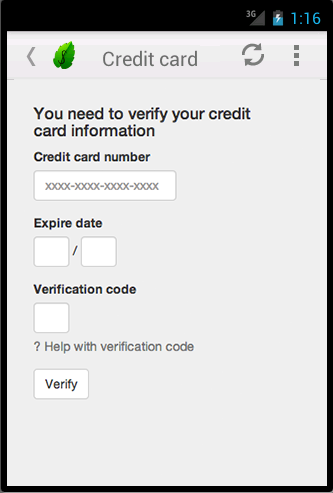
\includegraphics[width=2in]{./images/mint-example.png}
  \caption{Example of clickjacking attack on the Mint app.}
  \label{fig:mint}
\end{figure}

\textit{Mint} is designed to aggregate and present to users detailed reports of all their incomes and expenses from different financial sources.
The service produces the reports by periodically querying credit card and bank statements and by aggregating the transaction by time period and category.

The tool reported that one of Mint's activities is vulnerable to an \emph{entire screen} UI integrity attack, which results in showing to the user an arbitrary web page inside the application visual context. An attacker may exploit this vulnerability to create sophisticated clickjacking attacks~\cite{android-clickjacking}. An attack scenario consists in presenting to the user a crafted web resembling the Mint look and feel inside the Mint application.
In the page, the user is asked to reinsert her credit card details complete
with verification code because of identity verification purposes. Reasonably, the user would act as asked, since they already inserted such information in the Mint system.
The loaded web page is now free to send the collected credit card information to any server. It is also important to point out that the URL of the currently visualized page is never presented to the user. An example of this attack can be seen in Figure~\ref{fig:mint}.

\textit{Poste Pay} is a financial application by the Italian postal service company offered to manage the popular Poste Pay rechargeable debit card service. In the application, the user can access cards statements, recharge prepaid cell phones or even recharge any other Poste Pay card by users card credit. Using our approach, we were able to design a scam attack simulation by prompting messages to the users (i.e. an \emph{alert screen} UI integrity attack). Since the content of the message is completely specified by an attacker, a scenario could mimic traditional phishing attacks, prompting users to submit their information to a malicious website or email address. Another scenario could ask the user to make a one dollar transfer to a specific credit card in order to, for example, extend the expiration date of the card.

\textit{Booking} is the mobile application of the omonimous popular online hotel booking service, offering almost the same features as the website, such as
making a reservation, browsing hotels by geographical position, price and user rating. The reservation service relies on a valid credit card. A reservation is successful if the card credit pre-authorization goes through.

We found the application to be vulnerable, allowing attackers to fill arbitrary text in the ``Important Information'' screen in the Booking application (another instance of \emph{entire screen} vulnerability). An attack aimed to steal the reservation amount can be designed as follows. The user is informed of a (fake) server issue experienced by Booking itself, and told to proceed with a manual transaction to fake bank coordinates, or on an alternate (malicious) website.

\textit{GOSMS} is a popular SMS replacement client for Android. It supports theming, private inbox, spam blocking and a large range of custom emoticons. Thanks to our analysis, we were able to generate a \emph{user input} attack, by populating the SMS creation screen with arbitrary recipient and message body. An attacker may exploit this vulnerability, for instance, by creating a SMS fraud, pre-populating the user inputs with a fake demand for charity as SMS body. Then, (s)he fills in the recipient field a crafted paid number used to collect money from user's credit.

% \subsection{Defensive Applications}
% Here we want to describe a particularly interesting sample we came across
% while performing the analysis. In this case, the
% string solver was unable to define sample input strings that could go through
% the paths to the vulnerable sink.

% In the GoChat application we noticed a recurrent parameter included in the Intents
% exchanged between application components, also in cases not marked as vulnerable
% from the analyzer. The string solver was unable to find a solution for such
% parameter because of a constraint that we were not completely able to specify.
% Before marking this case as pathological, we went back to manually inspect the
% application decompiled code. By reconstructing a whole communication example
% between two application components we ware able to understand the reason why the
% analyzer failed in its execution. This parameter represents an authorization
% code exchanged between the sender and the receiver of the Intent to guarantee
% message sender authenticity. The exchanged code is compared by the receiver to
% the content of a intra-component same-application shared variable. If there a
% match is not encountered the execution of the sender is immediately stopped. We
% can compare this approach to the one used in web application exchanging CSRF
% tokens. Of course because of the randomness in the parameter, no static analysis
% technique would be able to guess the valid token.

% This solution is very effective in practice, since guarantees complete
% protection to application resources possibly exposed to Intent attacks by
% completely blocking the normal execution flow. Unfortunately this solution is
% not generalizable to the case in which the receiver is intended to be accessed
% by selected application. Because of application sandboxing, two different
% application can not share (or partially share) memory parts.

% Instead, in Twitter, we found a server-based authorization mechanism. We found 5
% potential network vulnerabilities in the application. In this application the
% marked Intent messages are decorated with an user token. This token is included
% in the request sent to the server. Of course, the request succeeds only if the
% transmitted token is a valid one. Also in this case statically determining a
% valid token is impossible.

% Differently to the solution presented earlier, this approach, relying on an
% external (trusted) resource, the application server, can fulfill requests for
% other applications that have already obtained valid server credentials. These
% credentials usually are exchanged as consequence of an OAuth session.
% Credentials given to third party applications can, usually, easily be revoked by
% the user itself from the application's server.

\subsection{Other experimental results}

\begin{table*}[t]
  \centering
  \begin{tabular}{|l|c|c|c|}
    \hline
    & Min & Max & Avg \\ \hline
    Per-application execution time & 2.4 min & 33.2 min & 12.3 min \\
    Per-application components & 3 & 31 & 24.5 \\
    Per-application vulnerable paths & 2 & 19 & 4.2 \\
    Per-path statements & 5 & 81 & 17.2 \\
    Per-path if-statements & 0 & 3 & 0.98 \\
    \hline
  \end{tabular}
  \caption{Other experimental setup}
  \label{table:other_experimental}
\end{table*}

In Table~\ref{table:other_experimental} we summarize several performance indexes, including information about analysis execution time, path lengths and components in the applications, and so on. As it can be noted, the execution time depends on the number of components of an application. The per-application
execution time range is very wide, varying from a minimum of 2.4 minutes for 3 analyzed components to a maximum of 33.3 minutes spent to analyze an
application including 31 components. The execution time is heavily dominated by the IFDS analysis which consists in 70-80\% of the overall execution time.
The whole analysis took 16.4 hours to complete with an average per-application execution time of 12.3 minutes.

We discovered 92 paths leading to a sink out of 537 analyzed with an average of 4.2 vulnerable paths per application. For each vulnerable path the analyzer collected an average number of 17.2 statements with an average number of 5.8 statements including API calls. We approximated the 31.2\% of the supported API methods by not giving precise formulations due to Kaluza limitations, as described in Section \ref{section:kaluzaTranslation}. We found this not to be a limitation to our approach for two reasons: this apparently large number of approximations were performed, in practice, over the 7.7\% of the total number of translated statements including API calls, meaning that approximated transformations are, in general, infrequent.
Second, it is worth noting that within the analyzed paths, very few include validation checks over the data in input. In particular, our tool found at most 3 checks in those paths, usually checks on null values. In short validation checks involving Intent payloads are performed in the 23\% of the vulnerable paths.

\subsection{Discussion of Results and Recommendations}

From our results, it is clear that only a few applications properly implement validation of data received from Intent messages. Most applications perform only basic checks on Intent payloads parts, such as null-checks, performed only to protect against malformed Intents payload tuples. Such checks are not strict enough to defend application resources against more sophisticated Intent spoofing attacks as the ones we considered in this work.

In order to verify the intents' origins, currently developers may need to implement custom authentication mechanisms, given the absence of a system-provided intent origin verification feature. A recommended solution consists in exchanging keys between intent sender and receiver, and requiring signatures to be exchanged within intents as a mean of authentication. This solution is very similar to the one used in web application exchanging CSRF tokens, and it is very effective in practice, since it guarantees complete protection to application components possibly exposed to Intent attacks. However, it requires communication of key material among applications before normal communications can start.
% this solution is
% not generalizable to the case in which the receiver is intended to be accessed by selected application. Because of application sandboxing, two different application can not share (or partially share) memory parts.

An OS-level enhancement to offer to final users a set of features
in the Intent API to reliably retrieve an intent's origin or sign intent's data would also help mitigate this risk. A work that proposes something similar can be found in~\cite{quire2011}.
% Offering such features means in practice to insert in the environment an additional trusted entity
% in charge of generating and validating communication signatures. An encrypted communication channel with a verified remote server may also help in solving this problem, even though it would not be practical.

Most importantly, developers should always include strong data validation checks, even when dealing with intents, and should follow all the guidelines to securely implement intent communications by not exposing their application components unnecessarily.
